\documentclass[english]{tktltiki}
\usepackage[pdftex]{graphicx}
\usepackage{subfigure}
\usepackage{url}
\usepackage[usenames,dvipsnames]{xcolor}
\usepackage{listings}
\begin{document}
%\doublespacing
%\singlespacing
\onehalfspacing

\lstdefinelanguage{Ini}
{
    basicstyle=\ttfamily\small\singlespacing,
    columns=fullflexible,
    morecomment=[s][\color{Orchid}\bfseries]{[}{]},
    morecomment=[l]{\#},
    morecomment=[l]{;},
    commentstyle=\color{gray}\ttfamily,
    morekeywords={},
    otherkeywords={=,:},
    keywordstyle={\color{red}\bfseries}
}

\title{Browsing webs and playing games using an eye tracker: practical issues}
\author{Liangyi Luo, Tomi Simsiö, }
\date{\today}

\maketitle

\numberofpagesinformation{\numberofpages\ pages + \numberofappendixpages\ appendices }
%\classification{\protect{\ \\
%x.x [Human-centered computing],\\
%x.x.x [Interaction design]}}

\keywords{ }

\begin{abstract}

TBA

\end{abstract}

\mytableofcontents




\section{Introduction}

This is the report on the project about eye tracking for the course Interface Technologies in the Autumn of 2015. In this report, we present our project that intends to demonstrate the concepts and explore issues of using Eye Tracking technologies to augment gaming and web browsing experience.  

The model of the eye tracker used is Mirametrix S2. The technology Mirametrix S2 based on is called Infrared Pupil-Corneal Reflection Tracking (IR-PCR), which is one of the most widely used video-based eye tracking technologies. 

In Section 2, there is a succinct introduction to video-based eye tracking in general as well as idiosyncrasies of IR-PCR in the first place, which is followed by a brief review of existing applications of eye tracking technologies. Then in Section 2, known advantages and problems of the IR-PCR technology in current applications will be briefly discussed. Lastly, there is an overview of the composition of the test platform.

There are two subjects of interest in the project, thus two program prototypes were made: a Google Chrome extension and a game (controller) framework.  Both prototypes used the eye tracker as a means of interface control.

Section 3 reports the Chrome extension and Section 4 reports the game framework. In both Section 3 and Section 4, the motives and ideas for applying an eye tracking technology to the relative interface will be elaborated in the first place. Then, there will be a brief introduction to the composition and working principle of the prototype. This is followed by an illustration of usage with some skatchings/screenshots. 

In Section 5,  an analysis on practicality of using IR-PCR technology for web browsing and for controlling game is presented. Then, we summarize what we have learned during the project work.


\section{Video-based eye tracking}

\subsection{A brief introduction to video-based tracking}

On the retina of a human eye, there is a small pit shaped structure called "fovea centralis", where the density of cone cells is significantly higher than the rest of the retina. Cone cells enable a human's colour vision in well illuminated environments. Fovea centralis grands the sharp central vision, whereas the rest of retina provides much less sharp peripheral vision. The visual field of a normal human being is more than one hundred and eighty degrees, in which the fovea centralis can covers about one degree only. A human has to move its eyes thus move the point of regard in order to acquire clear vision from multiple directions. Therefore, images of eye movements can be used to track a human's points of regard.

Video-based eye tracking technologies use images of eyes as raw data to compute the corresponding points of regard. A video-based eye tracking system usually consists of a camera and a computer system with adequate software that measures relative movements of eyes from images captured by the camera. Usually, the displacements of pupils are used to track eyes' relative movements, which can be mapped to movements of points of regard through a calibration process. 

The performance of a video-based eye tracking system is limited by its hardware and software. The camera is the most important hardware component in an eye tracking system. The maximum resolution of the images captured by the camera determines maximum precision of measurements of eye movements. Moreover, the maximum frame rate determines the sample rate of eye movements. This is important because that human eyes have rapid micro movements called "saccades" when gazing at something. Smoothing techniques are required to acquire the point of regard from saccades. Thus, higher sample rates of saccades help track the point of regard. As for the software, essential tasks for tracking eye movements, such as the calibration, computation, as well as some error compensations are all handle by the software. 


\subsection{Infrared Pupil-Corneal Reflection Tracking}

Infrared Pupil-Corneal Reflection Tracking (IR-PCR) is one of the most popular eye tracking technologies. IR-PCR eye trackers shoot infrared light towards human eyes then use the reflection to track eye moments. There are two alternatives of IR-PCR: bright pupil tracking and dark pupil tracking. A "bright pupil" eye tracker's camera is on the path of the reflection, such that the infrared light reflected back from the retinas will enter the camera lens. In the images captured by the camera, the pupils are illuminated and appear to be bright white discs. A "dark pupil" tracker's camera avoids the path of the retinal reflection, such that the pupils are darker than irises and limbi and appear to be dark discs. Either way, the pupils are highlighted and rendered easier to track. In addition to highlighted pupils, corneas of eyes will reflect the infrared light source as bright light spots, despite the position of eyes, due to corneas' hemisphere shape. Using the bright spot as reference objects, the relative positions of pupils can be tracked, hence the eye movements are known.


\subsection{A review of applications}

There are plenty applications of eye tracking technologies. Generally speaking, an application may use eye trackers for interactions or merely observations. The former case is more often seen in human-computer interactions whereas the later is in studies and researches. 

According to users' awareness of and control over the tracking process, applications of eye tracking can be put into four categories according to Majaranta and Bulling.\cite{majaranta14}

The first category is called "explicit eye input", where a user interacts with an interface by voluntary control using gazing, blinking, or even head movements, given that some device can track head movements. In this category, some applications use only eye-based control for special use cases while other implement multimodal control to avoid the "Midas touch" problem \cite{Velichkovsky97}

On the "eye-based only" side, some interesting applications are: interfaces featuring gaze gestures\cite{Drewes:2007:ICU:1778331.1778385}\cite{Ohno:1998:FEG:786112.786297}; a "hand-free" web browser\cite{5090980}; a gaze-based text input\cite{wardmackay2002}, which can achieve an input rate of 29wpm; a smartwatch interface\cite{Hansen:2015:GIT:2800835.2804332}. "Eye-based only" control technology is generally useful in scenarios where using hands are not an option. It is extremely beneficial for people with physical disabilities in hands or arms. 

On the multimodal side, some interesting applications are: multi-modal user interface\cite{538404}\cite{maglio2000}; gaze controlled games\cite{Isokoski:2009:GCG:1667488.1667491}. 

The second category is called "attentive user interfaces", where a user does not issue gaze-based commands over interfaces directly, nonetheless the system will still react to users' eye movements. Some interesting applications are: interactive movies\cite{doi:10.1080/14626260500476523}; interactive stuffed-toy\cite{Yonezawa:2007:GBS:1322192.1322218}.

The third category is called "gaze-based user modeling", where the goal is to discern patterns of user behaviors on an interface, or to assess an interface by doing so. Interesting application are mostly researches in human-computer interaction, human cognition, or psychology. Some examples are: usability research in human-computer interaction \cite{Poole05eyetracking} \cite{Jacob2003573}; visual perception research\cite{John2004}.

The fourth category is called "passive eye monitoring". This is the case in which data of eye movements are collected for study or inspection. There is no interaction in the process. No connection between eye movements and an interface will be established. An interesting example is about court tests on whether a driver is intoxicated during driving by monitoring eye movements\cite{Busloff1993}.

We actually found many concrete examples of applications, those in gaming control were especially interesting since one of our alternative idea for the project is about gaze controlled games. Videos of these examples can be found in the appendix. 

\subsection{Advantages and problems in using an IR-PCR eye tracker}

The Mirametrix S2 we are working with is a "bright pupil" IR-PCR eye tracker. Because an IR-PCR eye tracker generates its own reference points for tracking eyes, it does not require a user's head to stay absolutely still. Certain levels of flexibility on head movements is allowed. Besides, a binocular eye tracker that tracks both eyes of a user may be able to output data on users' head position based on the relative position of two eyes. The Mirametrix S2 eye tracker series happen to have this capability. This suggests that there is potential in using head gestures such as tilting head to enrich the means of control over the interface. 

On the latent problems of "bright pupil" eye tracker. Such eye trackers, which rely on the "bright pupil effect" to work, may perform differently on different individuals, due to the reason that the "bright pupil effect" isn't the same on every human \cite{Nguyen:2002:DIB:507072.507099} There could exists an inconsistency on tracking accuracy from different users even with the same device and calibration process. This actually agrees with our initial test on the Mirametrix S2 eye tracker. Considering this latent problem as well as the potentially wide user groups of the application, the software end of our system should has high error tolerance.

We are going to face some common problems of video-based eye tracking technologies too. The toughest nut might be the "Midas touch" problem.\cite{Velichkovsky97} In a "eye-based only" browser or game control system, "Midas touch" may result in unwanted operations. A possible countermeasure is using gaze gestures. \cite{Ohno:1998:FEG:786112.786297} However, more complicated gestures are needed to bring greater variations in control inputs, yet complicated eye gestures are not natural and bring fatigue. Moreover, an eye tracking device needs to be specifically positioned in order to perform with best possible accurracy. This can be probematic for laptop users.  Furthermore, calibration is required every time before use for every user. This isn't ideal for a browsing application that will be used often. Besides, the are several relatively minor problems. Users who wear spectacles or has droopy eyelids may find an eye tracker difficult to use. Some eye trackers might be sensitive to ambient light. 

\subsection{An overview of the system composition}

Our system consists of a Mirametrix S2 eye tracker, a virtual machine (server) with Windows OS and the system software for the eye tracker, and two prototypes ,id est Google Chrome plug-in and game control framework, to be tested. 

The Mirametrix S2 used for the project is an IR-PCR eye tracker. The official specification states that it has accuracy of less than one degree of visual angle. The "data rate" is 60Hz, means it captures an image of eyes, compute coordinates, and output x,y coordinate as floating points in range [0,1] 60 times per second. It is capable of binocular tracking, which suggests that tilting heads can be detected. It allows head motion in a 25cm width , 11cm height window with 30cm depth. The recommended distance between a user and the device is 65cm. That gives us 50cm to 80cm distance flexibility in a 25x11cm window. 

The software suit provided by the device manufacture, of which the server software and the driver are most crucial, runs only on Windows machines (including virtual machines). Hence aforementioned Windows virtual machine was used as a server that streams data from the eye tracker. With the server running, we can communicate with the device using TCP/IP protocal from a computer with operation systems other than Windows. In the project, the host computer is a laptop with Linux. 

Through some initial test of the device, we realized that the accuracy stated in the device specifications, presumably achieved in controlled tests, was not our case. This actually agreed with what we learned about accuracy of eye trackers in practice from literature. \cite{majaranta14} However, inaccuracy should be taken into account for eye tracking technology in web browsing and game controling applications no matter what is the capability of the device used.


\section{The implementation for web browsing: a Google Chrome browser plug-in with an eye tracker}


\subsection{The motives and ideas for the interface}  

In a searching task, in which a user is browsing through large amount of web pages to find something, it will be convenient if the user can preview a web page with a given link because the link might not contain enough information to indicate the interestingness of the corresponding web page. Moreover, the user might need to constantly switch between selecting and viewing, which requires mouse input, and text entering, which requires typing with both hands on a keyboard. According to the Fitts' Law and the Keystroke-level modal,\cite{Fitts64}\cite{Card:1980:KMU:358886.358895} pointing and selecting as well as the reciprocating motion of a hand between keyboard and mouse take time. 

Based on the premises and assumptions above, what we can think of is a browsing mechanism that uses an eye tracker instead of a mouse as a pointing device. Besides, it has a preview function that opens a preview windows for the link the user pointed at. Therefore the project focus on the idea of pointing and previewing using an eye tracker.  



\subsection{The composition and working principle of the plug-in}

{illustration}
\begin{figure}[h]
%\begin{figure}[tbh] t= top, b = bottom, h=here
\ \newline
\begin{center}
%\includegraphics[width=0.9\textwidth]{kuvaesimerkki.pdf}
%\rotatebox{90}{\includegraphics[scale=.75]{kuvaesimerkki.pdf}}
\caption{Figure elements.}
\label{kuvaesimerkki}
\end{center}
\end{figure}

\subsection{An illustration of the usage of the interface}

{illustration}
\begin{figure}[h]
%\begin{figure}[tbh] t= top, b = bottom, h=here
\ \newline
\begin{center}
%\includegraphics[width=0.9\textwidth]{kuvaesimerkki.pdf}
%\rotatebox{90}{\includegraphics[scale=.75]{kuvaesimerkki.pdf}}
\caption{Figure elements.}
\label{kuvaesimerkki}
\end{center}
\end{figure}

%\pagebreak



\section{The implementation for gaming: Using an eye tracker as a game controller}


\subsection{The motives and ideas for the interface design}

Certain genres of games such as Simulation and Real-Time Strategy requires navigating the view window/camera towards different directions of the map. This is traditionally done by a clicking or moving mice or press arrow keys. With an eye tracker, we might explore more possibilities in keyboard-and-mouse control if hands are free from view navigation. 


\subsection{The composition and working principle of the game controller framework}

Our game controller framework aims to provide easily configurable camera-movement controlling for all games that have a camera, which is moved by either arrow-keys or WASD-keys. When the user looks to a side of the screen, our controller framework emulates keyboard keypress to move camera in that direction. For example, when the user looks to close of the left border of the screen, our framework emulates left arrow or A-key press to move the camera leftwards. Keypress emulation is done via the uinput kernel module.

Every game has different 2D user interface and thus every game needs a different configuration to specify when and how to move the camera. This is done in our framework with game-specific configuration files. Listing \ref{gcfconf} is an example of such file.

We got up to 60 gaze-events per second from the eye tracker each telling where this user is looking at that moment. We reference to these events as ticks. The first configuration variable \verb|ticks_needed| defines how long the user needs to look at the side of the screen before the camera is being moved. The second variable \verb|action_every_ticks| specifies how many ticks to wait between emulated keypresses when the user keeps looking at the side of the screen. The movement happens by either arrow or WASD-keys, defined by the \verb|move_method|-variable.

The \verb|*_start| and \verb|*_margin|-variables define where the user needs to look in order to move the camera. The values are percentages of the screen. Horizontally left border of the screen is 0 and right border is 1. Vertically top border is 0 and bottom border is 1. So for example \verb|left_start = 0.2| means that when user is looking at somewhere on the leftmost fifth of the screen, the camera is being moved left. The \verb|*_margin|-variables may be helpful to rule out some possible 2D UI-bars on the sides of the screen. \verb|left_margin=0.0|, \verb|right_margin=1.0|, \verb|up_margin=0.0| and \verb|down_margin=1.0| means that no margins are in use.

\bigskip
\begin{lstlisting}[language={Ini},caption={Example of game-specific configuration file},label={gcfconf}]
[Camera]
# Number of subsequent ticks needed to make action
ticks_needed = 1
# How many ticks to wait between actions
action_every_ticks = 1
# How to move the camera? 'wasd' or 'arrows'
move_method = wasd

# Points when to start moving camera
left_start = 0.2
right_start = 0.8
up_start = 0.2
down_start = 0.75

# Reserve a margin where eg. infobars are
left_margin = 0.0
right_margin = 1.0
up_margin = 0.0
down_margin = 0.9
\end{lstlisting}
\bigskip

The game controller framework is used with command \verb|python main.py|. This lists all available game configurations. Controlling can be started with e.g.\newline \verb|python main.py -g cities_skylines|.

\subsection{An illustration of the usage of the interface}

Figure \ref{citiesskylines} illustrates where the user needs to look while playing Cities Skylines with configuration from listing \ref{gcfconf}. Camera will move up while looking at the top red area, down while looking at the bottom red area and sideways while looking at the blue areas. Vertical an horizontal movement can happen simultaneously. Cities Skylines has a toolbar on the bottom of the screen, so that area is ruled out by setting \verb|down_margin=0.9|.

\begin{figure}[h]
\begin{center}
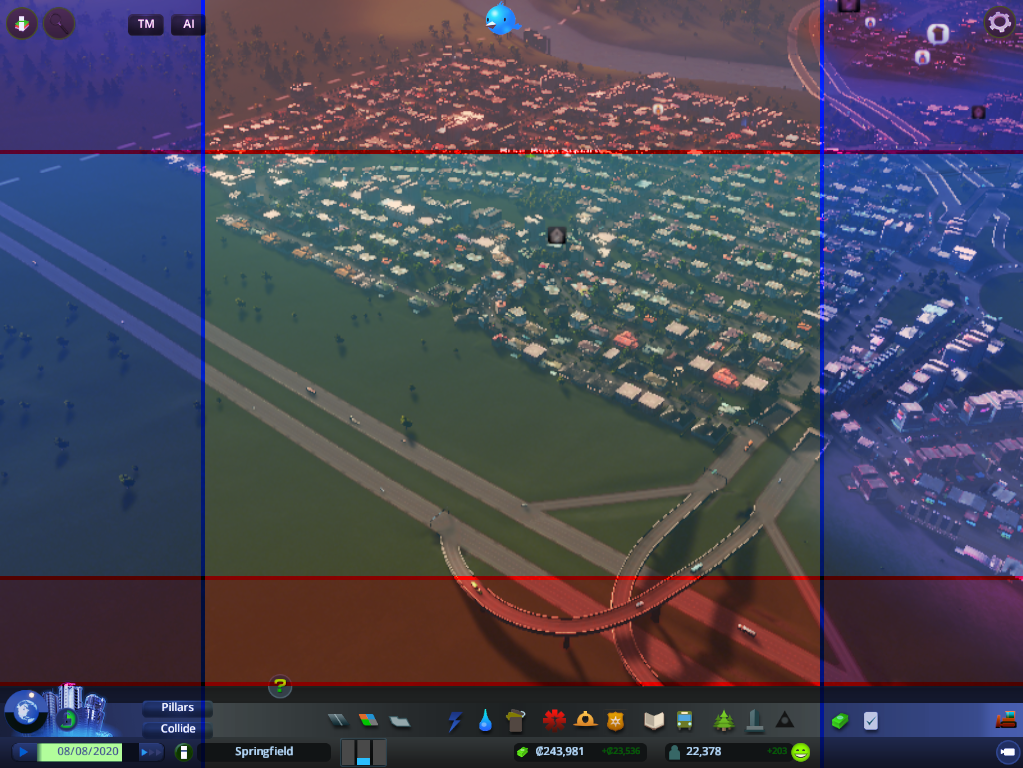
\includegraphics[width=1\textwidth]{cities_skylines.png}
\caption{Relevant screen sections highlighted over a screenshot from Cities Skylines}
\label{citiesskylines}
\end{center}
\end{figure}



\section{Discussion}

\subsection{Practicality analysis}

Several issues became conspicuous during the test of the prototype. 

Firstly, accuracy issues were major issues in both prototypes. In the test of the Chrome extension, the test subject had difficulties in pointing at links with small clickable logo size. In the test of the game control framework, navigating upwards did not work well. This wasn't so surprising since our earily test had already exposed the issue about inaccurate pointing. On the negative side, this might be a bigger issue in practice given that the positioning and calibration of a device could be worse than the condition in our test. For web browsing, inaccuracy leads to the requirement for bigger clickable logos. Besides, inaccurate pointing may result in unwanted previewing or opening the wrong web page. This could be more or less an issue that depends on the specific browsing task. For controlling games, less accuracy means less available operations for eyes to commence. Because most pointing operations in games are originally based on mouse pointing or at least joystick pointing, both are more accurate than current eye trackers.

On the positive side, problems about inaccuracy are device dependent, suggesting that eye pointing can be practical if there exist eye trackers that perform as well as mice as pointing devices. Therefore, the ideas of using eye tracking in web browsing or controlling game work or not is relying on the advancement of eye tracking technologies. To think in a different angle, even if the accuracy of eye tracking technologies can hardly be improved yet the need for such technologies is rigid, then the interfaces of required applications can adapt. A reference case for web browsing is that many websites provide web pages customised for small screens of mobile phones. The situation for eye trackers is different from mobile phones. Eye tracking technologies are not required for most browsing and it is even harder to find a case where eye trackers are absolutely necessary. Expecting eye trackers to become as ubiquitous as mobile phones is unrealistic. Likewise, games that use eye trackers are minority because most players are content with mice, keyboards, and joysticks. Nevertheless, there might be more hope to see a burgeoning use of eye trackers in games because eye trackers indeed have the potential to provide interesting features in games such as eye contact with a non-player character. Most importantly, such features in games might work with compromised accuracy.

All in all, why eye trackers are not practical for browsing tasks currently is that they are not required in most cases; however in games, the practicality of eye trackers is related to new and interesting interactions that are not accuracy demanding. Eye trackers are hitherto not practical in terms of accuracy. Eye trackers may become practical in the future if advancement of the eye tracking technologies resolve the inaccuracy issues or the need from users become essential.

Secondly, certain details decide the practicality of using eye trackers. Given the same idea for an interface, details in the implementation determines the user experience. In our tests, the delay before opening a preview or navigating towards a direction was a detail that required attention. We used semi-arbitrary values according to our intuitions; however in practice, such detail may require researches and experiments in order to acquire a "good" setting. Therefore, tuning an entire interface that contains multiple technical details may require a considerable amount of resources. This suggests that the practicality of using an eye tracking technology in web browsing or controlling games depends on how current technologies are used as well.

Thirdly, some inevitable problems in using the device were expected during the test. We commenced calibrations before each test and the body of the test subject needed to remain motionless during the test. These problems are also technology dependent. A calibration-free eye tracker with a large reception field was devoid of such problems; nonetheless,  the reasons for developing eye trackers with such features are still not strong enough to attract investments as such features are not usually required in controlled experiments yet casual users do not need eye trackers for most activities.


\subsection{Things we learned}



\subsection{Conclusion}



%\enlargethispage{5mm}

%\subsection{}

%\subsection{}

%\enlargethispage{5mm}



%\nocite{*}
\bibliographystyle{tktl}
\bibliography{lahteet}

\lastpage

\appendices

\pagestyle{empty}

\internalappendix{1}{Videos about eye tracking applications}

Most videos feature Tobii devices due to the fact that Tobii is one of the major eye tracking device manufactures.

"BMX rider Stephen Murray controls his computer with only his eyes"
https://www.youtube.com/watch?v=b\_wsnc8IdCQ

"Demo of Tobii EyeX in Gaming"
https://www.youtube.com/watch?v=oSo8fbZfHLk

"Gaze control of StarCraft2"
https://www.youtube.com/watch?v=s4ZCQ-jZxyE

"Tobii Gaze Interface for Windows 8 Revolutionizes Computer Interaction"
https://www.youtube.com/watch?v=3MoGzTdQnX8

\end{document}


